\documentclass{beamer}

\usepackage[utf8x]{inputenc}

\title{Energy Harvesting}
\author{Author: Miha \v Can\v cula \\
  Advisor: doc. dr. Du\v san Ponikvar}

\renewcommand{\vec}{\mathbf}

\institute{Faculty of Mathematics and Physics \\ University of Ljubljana}
\date{January 4, 2012}

\begin{document}

\frame{\titlepage}

\section{Introduction}

\begin{frame}
  \frametitle{Energy Harvesting}

\begin{block}{Definition}
  \begin{itemize}
    \item Self-powered devices
    \item Small amount of power \\ from the immediate environment
    \item Grid independence
  \end{itemize}
\end{block}

\begin{block}{Use-cases}
  \begin{itemize}
    \item Wireless sensors
    \begin{itemize}
      \item{Intelligent buildings}
      \item{Fire detection}
      \item{Pollution monitoring}
    \end{itemize}
    \item Consumer electronics
  \end{itemize}
\end{block}

\end{frame}

\begin{frame}
  \frametitle{Requirements}
\end{frame}

\begin{frame}
  \frametitle{Important characteristics}
\begin{block}{Electric}
\begin{itemize}
  \item Source resistance
  \item Open-circuit voltage $V_{oc}$
  \item Short-circuit current $I_{sc}$
  \item $V(I)$ curve and power curve
\end{itemize}
\end{block}

\begin{block}{Physical}
\begin{itemize}
  \item Efficiency
  \item Size and weight
  \item Cost
\end{itemize}
\end{block}

\end{frame}

\section{Photovoltaics}

\begin{frame}
  \frametitle{Photovoltaic cells}
\begin{itemize}
  \item Most used today
  \item Produce the most power
  \item Variable output
\end{itemize}

\end{frame}

\begin{frame}
  \frametitle{Theory}
\begin{columns}
  \begin{column}{.6\textwidth}
    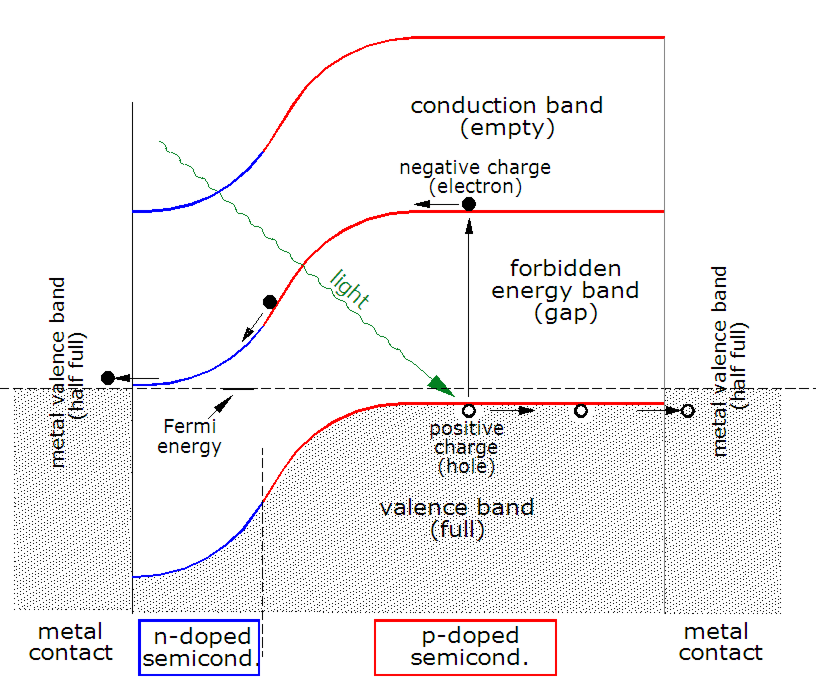
\includegraphics[width=\textwidth]{./Slike/PV-band-diagram}
  \end{column}
  \begin{column}{.4\textwidth}
    \begin{block}{Photovoltaic effect}
    \begin{itemize}
      \item Photon excites electron, creates electron-hole pair
      \item Electron moves to n-doped side
    \end{itemize}
    \end{block}
  \end{column}
\end{columns}

\end{frame}

\begin{frame}
  \frametitle{Characteristics}
  \begin{itemize}
    \item Efficiency $\sim$ 30\%
    \item Low $V_{oc}$ $\Rightarrow$ connected in series
    \item Close to ideal current source
  \end{itemize}
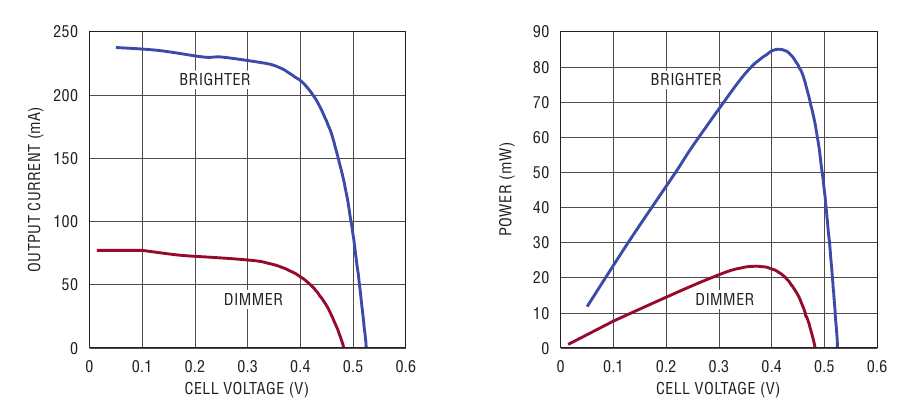
\includegraphics[width=\textwidth]{./Slike/PV-power-curve}


\end{frame}

\section{Thermoelectrics}

\begin{frame}
  \frametitle{Thermoelectric generators}
\begin{block}{Operation}
\begin{itemize}
  \item Electricity from tempareture gradient
  \item Cheap, simple and reliable
  \item Also used as coolers
\end{itemize}
\end{block}

\begin{block}{Heat sources}
  \begin{itemize}
    \item Waste heat from machines
    \item Buildings
    \item Body heat
  \end{itemize}
\end{block}


\end{frame}


\begin{frame}
  \frametitle{Theory}
\begin{columns}
  
\begin{column}{.5\textwidth}
\begin{block}{Seebeck effect}
  \begin{itemize}
    \item Thermocouples
    \item Directed diffusion of charge carriers
    \item Reversible
    \item Strongest in semiconductors
  \end{itemize}
\end{block}
\end{column}

\begin{column}{.5\textwidth}
\begin{block}{}
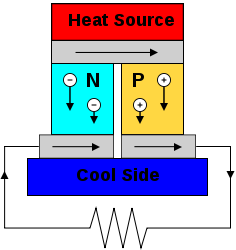
\includegraphics[height=150pt]{./Slike/TEG-couple}
\end{block}
\end{column}
\end{columns}
\end{frame}

\begin{frame}
  \frametitle{Characteristics}
\begin{itemize}
  \item $V_{oc}$ and $R$ grow linearly with number of couples
  \item Linear $V(I)$ curve

\begin{center}
  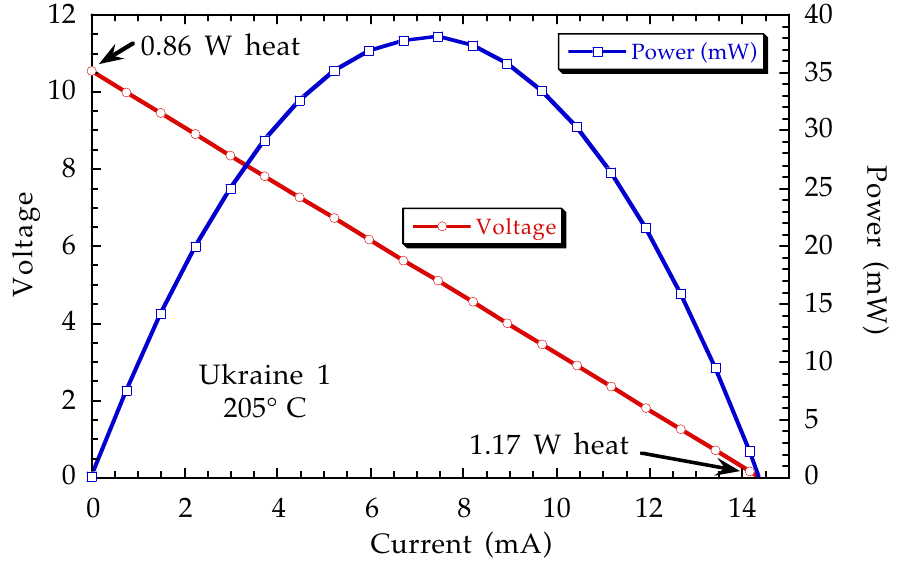
\includegraphics[height=120pt]{./Slike/TEG-curve}
\end{center}
 
\end{itemize}

\end{frame}



\section{Piezoelectrics}

\begin{frame}
  \frametitle{Piezoelectric generators}
\end{frame}

\begin{frame}
  \frametitle{Theory}

\begin{itemize}
  \item Crystalline materials
  \item Asymmetric unit cells
  \item Coupled Hooke's law and dielectric response
  \begin{align*}
 \vec S &= s \vec T + d^t \vec E \\
 \vec D &= d \vec T + \varepsilon \vec E
  \end{align*}
  \item Piezoelectric matrix $d$ is generally sparse
  \item Reversible
\end{itemize}


\end{frame}

\begin{frame}
  \frametitle{Characteristics}
\begin{itemize}
  \item High voltage $V_{oc}$
  \item Constant power curve
\end{itemize}

\begin{center}
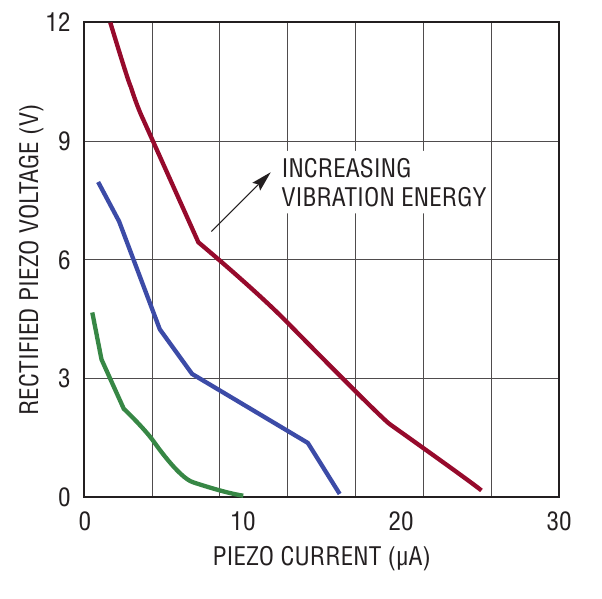
\includegraphics[width=0.5\textwidth]{./Slike/Piezo-UI}
\end{center}
  
\end{frame}

\section{Management and storage}

\begin{frame}
  \frametitle{Power management}
\end{frame}

\begin{frame}
  \frametitle{Energy storage}
\end{frame}

\section{Succesful implementations}

\begin{frame}
  \frametitle{Building automation}
\end{frame}

\begin{frame}
  \frametitle{Phone chargers}
\end{frame}

\section{Conclusion}

\begin{frame}{Conclusion}
  \begin{columns}
    \begin{column}{0.45\textwidth}
      \begin{block}{Uses}
        \begin{itemize}
          \item Wireless sensors
	  \item Batteryless electronics
	  \item Hard-to-reach places
        \end{itemize}
      \end{block}
      \begin{block}{Benefits}
        \begin{itemize}
          \item Low maintenance
	  \item Grid independence
	  \item Convenience
        \end{itemize}
      \end{block}
    \end{column}
    \begin{column}{0.5\textwidth}
      \begin{block}{Methods}
        \begin{itemize}
          \item Photovoltaic cells
	  \item Thermoelectric generators
	  \item Piezoelectrics
        \end{itemize}
      \end{block}
      \begin{block}{Power management}
        \begin{itemize}
          \item DC-DC converter
	  \item Storage element and charger
	  \item Batteries or ultracapacitors
        \end{itemize}
      \end{block}
    \end{column}
  \end{columns}
\end{frame}




\end{document}
